\setcounter{secnumdepth}{3}
\chapter{Software Design}
Dieses Kapitel widmet sich der Frage, was im speziellen Fall der Softwareentwicklung für Webseiten beim Design beachtet werden muss.

\section{Single Page Applications}
\label{sec:softwaredesign:singlepageapplications}
Die meisten Webseiten sind Multi Page Applications. Das bedeutet, dass eine neue Seite beim Server angefragt wird, wann immer er einen Link anklickt. Die Seite hat immer eine eigene Adresse über welche sie referenziert werden kann.

Bei \gls{spaLabel} wird initial eine Seite geladen und dann nicht mehr. Sobald ein Link angeklickt wird, geht zwar eine Anfrage an den Server, die Seite wird im Browser jedoch nicht neu geladen. Die Anfrage an den Server wird über JavaScript, im genaueren über \gls{ajaxLabel}, abgesetzt. Davon merkt der Benutzer jedoch nichts. Im Code sieht dies folgendermassen aus:

\begin{lstlisting}
var myAjax = new Ajax.Request(
  "datum.php",
  { method: 'get', onComplete: zeigeDatum }
);
\end{lstlisting}

In diesem Beispiel wird das prototype\footcite{Prototype_JavaScript_framework_a_foundation_for_ambitious_web_applications_2015-06-07} Framework verwendet, um eine Anfrage auf \textit{www.meineseite.com/datum.php} abzusetzen. Sobald die Antwort des Servers beim Browser eintrifft, wird die Methode \textit{zeigeDatum} aufgerufen.

Der Vorteil von \glspl{spaLabel} liegt darin, dass nur ein Teil der Webseite neu geladen werden muss. Sprich derjenige, welcher durch die Aktion verändert werden soll. Dadurch werden die Antwortzeiten der Benutzeraktionen minimiert.

Ein weiterer Vorteil liegt darin, dass der Server sich nicht um die Darstellung der Informationen kümmern muss, da dies vom Client erledigt wird. Der Server liefert nur Informationen aus, welche Anzuzeigen sind. Der Client entscheidet dann wie diese dargestellt werden sollen.

\glspl{spaLabel} haben jedoch auch einige Herausforderungen. Dadurch, dass die gesamte Seite nur eine Adresse besitzt, wird es schwieriger für Suchen, die Seite zu analysieren. Auch der Vor- und Zurück-Knopf der Browser funktioniert nicht mit \glspl{spaLabel}. Es gibt zwei Lösungen für das Problem:
\begin{itemize}
\item location.hash
\item pushState
\end{itemize}

In \Gls{glos:htmlLabel} gibt es Ankerlinks. Diese werden benötigt, um auf einer Seite an eine spezifische Stelle zu springen. Der Link \textit{www.meineseite.com} öffnet eine Seite. \textit{www.meineseite.com\#kontakt} zeigt die gleiche Seite an, springt jedoch zur Textstelle \textit{kontakt}. Es ist ein eigener Link und auch die History Funktion (Vor- \& Zurück-Button) des Browsers erkennt eine eigene Adresse. Der Browser lädt sich dabei jedoch nicht neu. Sprich diese Funktionalität kann für \glspl{spaLabel} verwendet werden. Dazu wird zum Beispiel folgender Link generiert: \textit{www.meineseite.com\textbf{\#}/products/fridge}. Die eigentliche Seite ist dabei \textit{www.meineseite.com} und es wird die Textstelle \textit{/products/fridge} angesprungen. Diese gibt es nicht auf der Seite, kann jedoch über \gls{jsLabel} nachgeladen werden.

Die neuere Möglichkeit, um \gls{seoLabel} für \gls{spaLabel} zu ermöglichen, ist die \textit{pushState} Funktionalität von \gls{jsLabel}.

\begin{lstlisting}
window.history.pushState(data, "Kühlschrank", "/products/fridge");
\end{lstlisting}

Dieser Aufruf setzt die Adresse des Browsers auf \textit{www.meineseite.com/products/fridge}, ohne die Seite dabei neu zu laden.

\section{Rich Internet Applications}
\glspl{riaLabel} sind Webseiten, welche einer dynamischen Desktopanwendung ähnlich sind. Dabei werden Drag-and-Drop, 3D-Effekte, Animationen und Unterstützung diverser Videoformaten ermöglicht. Zum Teil müssen \glspl{riaLabel} nicht zwingend in einem Browser ausgeführt werden, sondern benötigen lediglich Zugang zum Internet.

\begin{figure}[H]
	\centering
	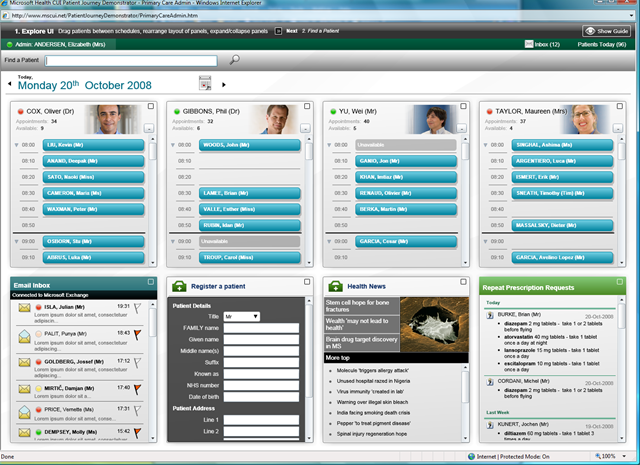
\includegraphics[width=.6\linewidth]{images/rich_internet_application.png}
	\caption{Beispiel für eine \gls{riaLabel}\footcite{AjaxWorld_Talk_Building_Rich_Internet_Applications_2015-06-07}}
	\label{fig:softwaredesign:richinternetapplication}
\end{figure}

Eine \gls{riaLabel} kann traditionell über \Gls{glos:htmlLabel} und \gls{jsLabel} funktionieren, oder über Plugins von drittanbietern laufen. Zum Beispiel Flash oder Java. Neue Trends zeigen, dass \gls{riaLabel} auf Basis von Plugins sukzessive durch \Gls{glos:htmlLabel} und \gls{jsLabel} abgelöst werden\footcite{Rich_Internet_Application_Market_Share_Global_Usage_2015-06-07}.

Der Vorteil besteht darin, dass das Look-and-Feel von bekannten Anwendungen aus dem Desktop Bereich übernommen wird, wodurch die Benutzerakzeptanz verbessert wird. Wenn ein Plugin verwendet wird, so werden auch die Problematiken, welche die verschiedenen Browser mit sich bringen, umgangen. 

Nachteilig dabei ist, dass das Laden der ersten Seite eventuell länger Dauert, da viele Elemente dargestellt werden müssen. Auch wird mehr Rechenleistung vom Client benötigt, was im speziellen einen Einfluss auf mobile Geräte haben kann. Auch gibt es dieselbe Problematik mit dem \gls{seoLabel}, wie sie im Abschnitt \ref{sec:softwaredesign:singlepageapplications} \nameref{sec:softwaredesign:singlepageapplications} beschrieben ist.